\startchapter{Modeling}
\label{chapter:Mod}
The goal of this modelling section is to 1) define the communication between two running programs. 2) design the communication identification strategy. 3) discuss the implementation of the communication methods in Windows 4) understand the dual-trace of two programs in the perspective of communication and how to retrieve the event information of the communications from the dual-trace  

With this model, it is able to decide how communications being identified from the dual-trace and how to present them to the user.

\section{Communication of Two Programs}\label{definition}
This section describe my understanding of communications happen between two running programs in the real world. The communication in this work is data transfer activities between two running programs through a specific channel. Some collaborative activities between the programs such as remote procedure call is out of the scope of this research. Communication among multiple programs (more than two) is not discussed in this work. The channel can be reopened again to start new communications after being closed. However, the reopened channel will be treated as a new communication. The way that I define the communication is leading to the communication identification in the dual-trace. So the definition is not about how the communication works but what it looks like. The definition of the communication consist of terminology and definition.

\subsection{Terminology}\label{term}
\textbf{Endpoint:}\\
An instance in a program at which a stream of data are sent or received (or both). It usually is identified by the handle of a specific communication method in the program. Such as a socket handle of TCP or UDP or a file handle of the named piped channel.\\
\textbf{Channel:}\\
A conduit connected two endpoints through  which data can be sent and received\\
\textbf{Channel open event:}\\
Operation to create and connect an endpoint to a specific channel\\
\textbf{Channel close event:}\\
Operation to disconnect and delete the endpoint from the channel.\\
\textbf{Send event:}\\
Operation to send a trunk of data from one endpoint to the other through  the channel.\\
\textbf{Receive event:}\\
Operation to receive a trunk of data at one endpoint from the other through the channel.\\
\textbf{Channel open stream:}\\
A set of all channel open events regarding to a specific endpoint.\\
\textbf{Channel close stream:}\\
A set of all channel close events regarding to a specific endpoint.\\
\textbf{Send stream:}\\
A set of all send events regarding to a specific endpoint.\\
\textbf{Receive stream:}\\
A set of all receive events regarding to a specific endpoint.\\
\textbf{Stream:}\\
A stream consist of a channel open stream, a channel close stream, a send stream and a receive stream. All of these streams regard to the same endpoint.


\subsection{Definition}
With the defined terminologies, a communication consist of two endpoints to a channel, each endpoint is corresponding to a stream. A stream contains one or more channel open events, one or zero send stream, one or zero receive stream and one or more channel close events. A visualized definition can be found in Figure\ref{communicationhappen}. The event numbers in this figure do not representing the exact number of a real communication but only an example. There are many communication methods for the data transfer communications, but all of them are compatible to this communication definition.

\begin{figure}[H]
\centerline{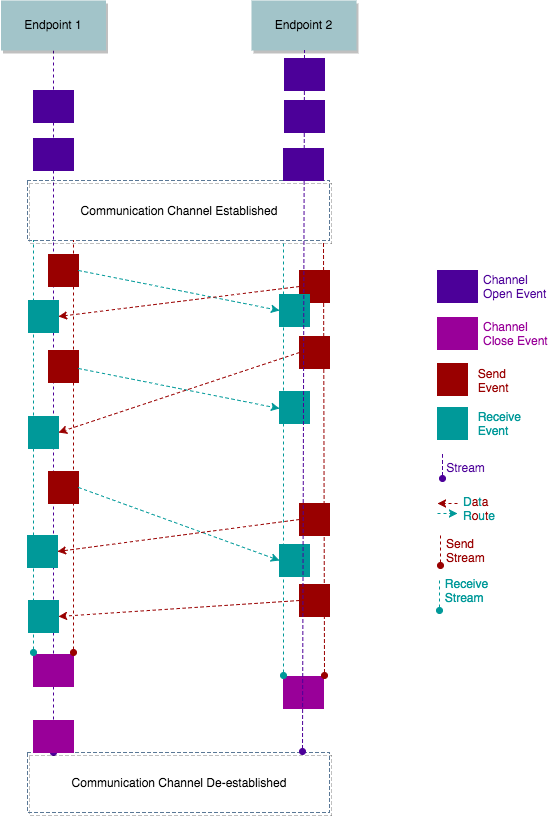
\includegraphics[scale=0.55]{Figures/communicationdefinition}}
 \caption{General Communication Model}
\label{communicationhappen}
\end{figure}


\section{Communication Categorization and Communication Methods}
This model divides all communication methods in two groups: reliable and unreliable communications. The reason to divide the communication methods into these two categories is that the send and receive streams or send and receive events matching strategies are respective for these two categories. In the first following two subsections, I summarize the characteristics of these two communication categories. The communication methods list in Table\ref{methodsInCategories} will be discussed further to provide more concrete comprehension. Not all communication methods in the real world are being leveraged in this thesis. However, this model is supposed to be applicable to other communication methods.
\begin{table}[H]
\centering
\caption{Communication Methods Discussed in This Work}
\label{methodsInCategories}
\begin{tabular}{|l|l|}
 \hline
\textbf{Reliable Communication}& \textbf{Unreliable Communication}\\
 \hline
Named Pipes & Message Queue   \\
TCP &  UDP \\
 \hline
\end{tabular}
\end{table}


\subsection{Reliable Communication}\label{reliable}
A reliable communication guarantees the data being sent by one endpoint of the channel always received lossless and in order to the other endpoint. With this property, the send data union in the send stream of one endpoint should equal to the receive data union in the receive stream of the other endpoint. The send data union is the conjunction of the data trunks in all send events in the send stream by the event time ordering. The receive data union is the conjunction of the data trunks in all receive events in the receive stream by the event time ordering. Therefore, the send and receive data verification should be in send and receive stream level by comparing the send data union of one endpoint to the receive data union of another. For some communication methods, a channel can be closed without waiting the completion of all data transmission. In this case, the receive data union can be a sub string of the send data union.

\subsection{Unreliable Communication}\label{unreliable}
An unreliable communication does not guarantee the data being send always arrive the receiver. Moreover, the data packets can arrive to the receiver in any order. However, the bright side of unreliable communication is that the packets being sent are always arrived as the origin packet, no data re-segmentation would happen. Accordingly, the send and receive data verification should be done by matching the data packets in a send event to a receive event on the other side.

\subsection{Communication Methods}
In this section, I describe the mechanism and the basic data transfer characteristics of each communication method in Table\ref{methodsInCategories} briefly. Moreover, data transfer scenarios are represented correspondingly in diagrams for each communication method. 
 
\subsubsection{Named Pipe}
In computing, a named pipe provides FIFO communication mechanism for inter-process communication. It allows two programs send and receive message through the named pipe.

The basic data transfer characteristics of Named Pipe are:
\begin{itemize}
  \item Bytes received in order
  \item Bytes sent as a whole trunk can be received in segments
  \item No data duplication
  \item Only the last trunk can be lost
\end{itemize}

Based on these characteristics, the data transfer scenarios of Named pipe can be summarized in Figure\ref{namedpipe}. 
\begin{figure}[H]
\centerline{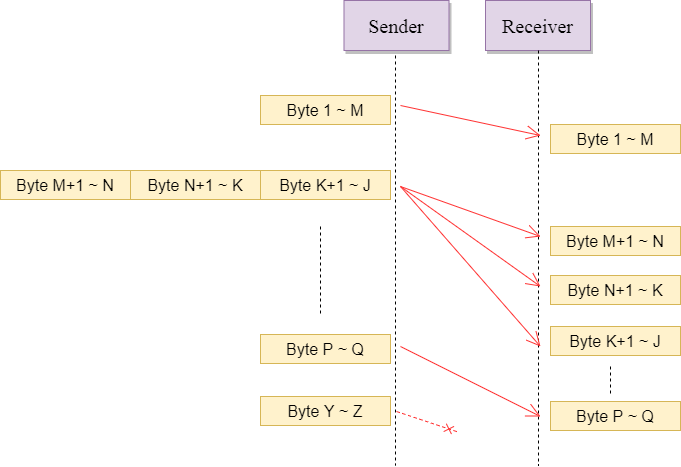
\includegraphics[scale=0.48]{Figures/namedpipe}}
\caption{Data Transfer Scenarios for Named Pipe}
\label{namedpipe}
\end{figure}

\subsubsection{Message Queue}
Message Queuing (MSMQ) is a communication method to allow applications which are running at different times across heterogeneous networks and systems that may be temporarily offline can still communicate with each other. Messages are sent to and read from queues by applications. Multiple sending applications can send messages to and multiple receiving applications can read messages from one queue.\cite{redkar2004pro} The applications are the endpoints of the communication. In this work, only one sending application versus one receiving application case is considered. Multiple senders to multiple receivers scenario can always be divided into multiple sender and receiver situation. Both endpoints of a communication can send to and receive from the channel.

The basic data transfer characteristics of Message Queue are:
\begin{itemize}
  \item Bytes sent in packet and received in packet, no bytes re-segmented
  \item Packets can lost
  \item Packets received in order
  \item No data duplication
\end{itemize}
Based on these characteristics,  the data transfer scenarios of Message Queue can be summarized in Figure\ref{msmq}.
\begin{figure}[H]
\centerline{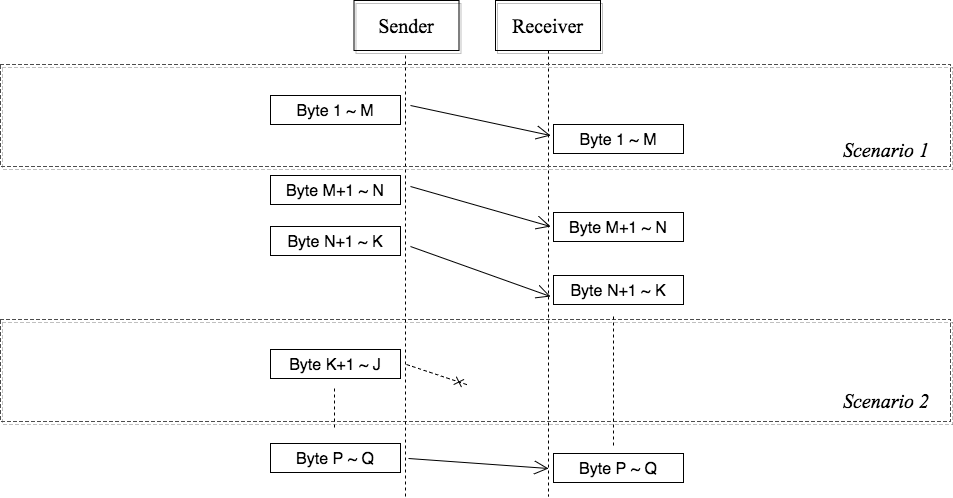
\includegraphics[scale=0.48]{Figures/msmq}}
\caption{Data Transfer Scenarios for Message Queue}
\label{msmq}
\end{figure}

\subsubsection{TCP}
TCP is the most fundamental reliable transport method in computer networking. TCP provides reliable, ordered, and error-checked delivery of a stream of octets between applications running on hosts in an IP network. The TCP header contains the sequence number of the sending octets and the acknowledge sequence this endpoint is expecting from the other endpoint(if ACK is set). The retransmission mechanism is based on the ACK. 

The basic data transfer characteristics of TCP are:
\begin{itemize}
  \item Bytes received in order
  \item No data lost(lost data will be retransmitted)
  \item No data duplication
  \item Sender window size is different from receiver's window size, so packets can be re-segmented
\end{itemize}

Based on these characteristics,  the data transfer scenarios of TCP can be summarized in Figure\ref{tcp}.
\begin{figure}[H]
\centerline{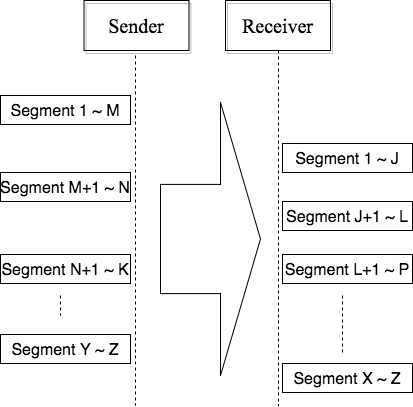
\includegraphics[scale=0.48]{Figures/tcp}}
 \caption{Data Transfer Scenarios for TCP}
\label{tcp}
\end{figure}

\subsubsection{UDP}
UDP is a widely used unreliable transmission method in computer networking. It is a simple protocol mechanism, which has no guarantee of delivery, ordering, or duplicate protection. This transmission method is suitable for many real time systems. 

The basic data transfer characteristics of UDP are:
\begin{itemize}
  \item Bytes sent in packet and received in packet, no re-segmentation
  \item Packets can lost
  \item Packets can be duplicated
  \item Packets can arrive receiver out of order
\end{itemize}

Based on these characteristics, the data transfer scenarios of UDP can be summarized in Figure\ref{upd}.
\begin{figure}[H]
\centerline{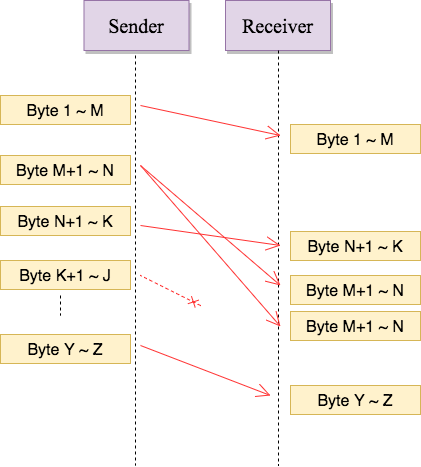
\includegraphics[scale=0.48]{Figures/udp}}
 \caption{Data Transfer Scenarios for UDP}
\label{upd}
\end{figure}

\section{Communication Identification Strategy}
In the first section of this chapter, I define what is a communication. The identification of the communications from a dual-trace should be able to identify the concerned communications as well as all the components defined in it. The section section in this chapter investigate the characteristics of the communication methods which is the key factor affecting the verification of the transferred data of a communication. From the trace analysis point of view, channel open events are essential to identify an endpoint while all other events are optional in the identification.

The identification contains seven major steps:
\begin{itemize}
 \item Locate all events
 \item Identify the endpoints from the channel open events
 \item Group the related events into streams, send streams and receive streams, then bind them to the corresponding endpoint
 \item Match the endpoints to the communications
 \item For reliable communication, verify if the send data union in the stream of one endpoint match the receive data union in the stream of the other endpoint; For unreliable communication, try to match the send and receive events of both endpoints 
 \item Construct and organize all the retrieved data of the communication 
 \item Present the identified communications to the user
\end{itemize}

\section{Communication Methods' Implementation in Windows}\label{windows}
In this section, the implementations of the four communication methods in Windows system are investigated. The goal of this investigation is to determine the system functions for the events in the communication definition and summarize the necessary parameters of all the communication events to further identify a communication. Each function call will be considered as an event. The channel opening mechanism is essential for identifying the endpoints and further the communication. Hence the channel opening mechanisms of each method are described in detail and represented in diagrams. 

I reviewed the Windows APIs of the communication methods and their example code. For each communication method, a system function list is provided for reference. These lists contain function names, essential parameters. These functions are supported in most Windows operating systems, such as Windows 8, Window 7. 

Windows API set is very sophisticated and multiple solutions are provided to fulfil a communication method. It is impossible to enumerate all solutions for each communication method. I only give the most basic usage provided in Windows documentation. Therefore, the provided system function lists for the events should not be considered as the only combination or solution for each communication method. With the understanding of the model, it should be fairly easy to draw out lists for other solutions or other communication methods. 

Moreover, the instances of this model only demonstrate Windows C++ APIs. This model may be generalizable to other operating systems with the effort of understanding the APIs of those operating systems.

\subsection{Windows Calling Convention}
The Windows calling convention is important to know in this research. The communication identification relies not only on the system function names but also the key parameter values. In the assembly level execution traces, the parameter values is captured in the memory changes of the instructions. The memory changes are recognized by the register names or the memory address. The calling convention helps us to understand where the parameters are stored so that we can find them in the memory change map in the trace.

Calling Convention is different for operating systems and the programming language. Based on the need of this work, we only list the Microsoft* x64 calling convention for interfacing with C/C++ style functions:\par
\begin{enumerate}  
\item RCX, RDX, R8, R9 are used for integer and pointer arguments in that order left to right.
\item XMM0, 1, 2, and 3 are used for floating point arguments.
\item Additional arguments are pushed on the stack left to right. \ldots 
\item Parameters less than 64 bits long are not zero extended; the high bits contain garbage.
\item Integer return values (similar to x86) are returned in RAX if 64 bits or less.
\item Floating point return values are returned in XMM0.
\item Larger return values (structs) have space allocated on the stack by the caller, and RCX then contains a pointer to the return space when the callee is called. Register usage for integer parameters is then pushed one to the right. RAX returns this address to the caller.
\end{enumerate}

\subsection{Named Pipes}
In Windows, a named pipe is a communication method for the pipe server and one or more pipe clients. The pipe has a name, can be one-way or duplex. Both the server and clients can read or write into the pipe.\cite{WinNamedpipe} In this work, I only consider one server versus one client communication. One server to multiple clients scenario can always be divided into multiple server and client communications thanks to the characteristic that each client and server communication has a separate conduit. The server and client are endpoints in the communication. We call the server ``server endpoint" while the client ``client endpoint".  The server endpoint and client endpoint of a named pipe share the same pipe name, but each endpoint has its own buffers and handles. 

There are two modes for data transfer in the named pipe communication method, synchronous and asynchronous.  Modes affect the functions used to complete the send and receive operation. I list the related functions for both synchronous mode and asynchronous mode. The create channel functions for both modes are the same but with different input parameter value. The functions for send and receive message are also the same for both cases. However, the operation of the send and receive functions are different for different modes. In addition, an extra function \textit{GetOverlappedResult} is being called to check if the sending or receiving operation finish, the output message will be stored in the overlap structure whose memory address saved in the function's output parameter Overlap Structure Address. Table\ref{synfunctions} lists the functions of the events for synchronous mode while Table\ref{asynfunctions} lists the functions of the events for the asynchronous mode for a Named pipe communication.

    \begin{table}[H]
        \centering
        \caption{Function List  of events for Synchronous Named Pipe}
        \label{synfunctions}
        \begin{tabular}{|l|l|l|l|l|}
            \hline
             \multirow{2}{*}{\textbf{Event}} &
               \multicolumn{2}{c|}{\textbf{Server Endpoint}} &
               \multicolumn{2}{c|}{\textbf{Client Endpoint}} \\
             \cline{2-5}
              & \textbf{Function}& \textbf{Parameters} & \textbf{Function} & \textbf{Parameters}  \\
             \hline
             \multirow{2}{*}{{\textbf{Channel Open}}}
             &\multirow{2}{*}{{CreateNamedPipe}} &  RAX: File Handler & \multirow{2}{*}{CreateFile} &  RAX: File Handler\\
              \cline{3-3} \cline{5-5}
             &&  RCX: File Name &  &  RCX: File Name\\
            \hline
             \multirow{3}{*}{{\textbf{Send}}}
             &\multirow{3}{*}{WriteFile} &  RCX: File Handle & \multirow{3}{*}{WriteFile} &  RCX: File Handle\\
              \cline{3-3} \cline{5-5}
             &&  RDX: Buffer Address &  &  RDX: Buffer Address\\
                           \cline{3-3} \cline{5-5}
             & &  R9: Message Length &  &  R9: Message Length\\
            \hline
             \multirow{3}{*}{{\textbf{Receive}}}
             & \multirow{3}{*}{ReadFile}&  RCX: File Handle & \multirow{3}{*}{ReadFile} &  RCX: File Handle\\
              \cline{3-3} \cline{5-5}
              &&  RDX: Buffer Address &  &  RDX: Buffer Address\\
                           \cline{3-3} \cline{5-5}
             & &  R9: Message Length &  &  R9: Message Length\\
            \hline
           {{\textbf{Channel Close}}}
             &{CloseHandle} & {RCX: File Handler} & {CloseHandle} & {RCX: File Handler}\\
            \hline
        \end{tabular}
    \end{table}

    \begin{table}[H]
        \centering
        \caption{Function List  of events for Asynchronous Named Pipe}
        \label{asynfunctions}
        \begin{tabular}{|l|l|l|l|l|}
            \hline
             \multirow{2}{*}{\textbf{Event}} &
               \multicolumn{2}{c|}{\textbf{Server Endpoint}} &
               \multicolumn{2}{c|}{\textbf{Client Endpoint}} \\
             \cline{2-5}
              & \textbf{Function}& \textbf{Parameters} & \textbf{Function} & \textbf{Parameters}  \\
             \hline
             \multirow{2}{*}{{\textbf{Channel Open}}}
             &\multirow{2}{*}{{CreateNamedPipe}} &  RAX: File Handler & \multirow{2}{*}{CreateFile} &  RAX: File Handle\\
              \cline{3-3} \cline{5-5}
             &&  RCX: File Name &  &  RCX: File Name\\
            \hline
             \multirow{3}{*}{{\textbf{Send}}}
             &\multirow{3}{*}{WriteFile} &  RCX: File Handle & \multirow{3}{*}{WriteFile} &  RCX: File Handle\\
              \cline{3-3} \cline{5-5}
             &&  RDX: Buffer Address &  &  RDX: Buffer Address\\
                           \cline{3-3} \cline{5-5}
             & &  R9: Message Length &  &  R9: Message Length\\
            \hline
            \multirow{3}{*}{{\textbf{Receive}}}
             & \multirow{3}{*}{ReadFile}&  RAX: File Handle & \multirow{3}{*}{ReadFile} &  RCX: File Handle\\
              \cline{3-3} \cline{5-5}
              &&  RDX: Buffer Address &  &  RDX: Buffer Address\\
                           \cline{3-3} \cline{5-5}
             & &  R9: Message Length &  &  R9: Message Length\\
              \hline
               \multirow{2}{*}{{\textbf{Receive}}}
             & \multirow{2}{*}{GetOverlapped-}&  RCX: File Handler & \multirow{2}{*}{GetOverlapped-} &  RCX: File Handler\\
              \cline{3-3} \cline{5-5}
             &  \multirow{2}{*}{Result} &  RDX:  Overlap  &  \multirow{2}{*}{Result }&  RDX:  Overlap \\
              &  &  Structure address &  &  Structure Address\\
            \hline                       
            \textbf{Channel Close}
             &{CloseHandle} &{RCX: File Handler} & {CloseHandle} &  {RCX: File Handler}\\
            \hline
        \end{tabular}
    \end{table}
    
A named pipe server is responsible for the creation of the pipe, while clients can connect to the pipe after it was created. The creation and connection of a named pipe returns the handle ID of that pipe. These handler Ids will be used later when data is being sent or received to a specified pipe. Figure\ref{namedpipeopen} shows the channel set up process for a Named Pipe communication.
\begin{figure}[H]
\centerline{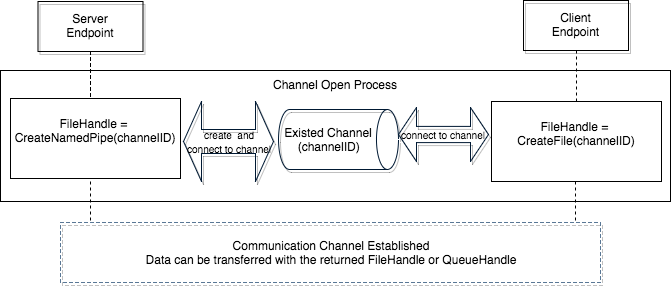
\includegraphics[scale=0.55]{Figures/namepipechannelopen}}
 \caption{Channel Open Process for a Named Pipe}
\label{namedpipeopen}
\end{figure}

\subsection{Message Queue}
Similar to Named Pipe, Message Queue's implementation in Windows also has two modes, synchronous and asynchronous. Moreover, the asynchronous mode further divides into two operations, one with callback function while the other without. With the callback function, the callback function would be called when the send or receive operations finish. Without callback function, the general function \textit{MQGetOverlappedResult} should be called by the endpoints to check if the message sending or receiving operation finish, the output message will be stored in the overlap structure whose memory address saved in the function's output parameter Overlap Structure Address. Table\ref{msmqsynfunctions} lists the functions for synchronous mode while Table\ref{msmqasynfunctionscallback} and Table\ref{msmqasynfunctions} list the functions for the asynchronous mode with and without callback. 

    \begin{table}[H]
        \centering
        \caption{Function List  of events for Synchronous MSMQ}
        \label{msmqsynfunctions}
        \begin{tabular}{|l|l|l|}
            \hline
             \textbf{Event} & \textbf{Function}& \textbf{Parameters}  \\
             \hline
             \multirow{2}{*}{{\textbf{Channel Open}}}
             &\multirow{2}{*}{{MQOpenQueue}} &  RAX: Queue Handler\\
              \cline{3-3} 
             & &  RCX: Queue Format Name\\
            \hline
             \multirow{2}{*}{{\textbf{Send}}}
             &\multirow{2}{*}{MQSendMessage} &  RCX: Queue Handle \\
              \cline{3-3} 
             &&  RDX: Message description structure Address \\
            \hline
             \multirow{2}{*}{{\textbf{Receive}}}
             & \multirow{2}{*}{MQReceiveMessage}&  RCX: Queue Handle \\
              \cline{3-3} 
              &&  R9: Message description structure Address \\
            \hline
            \textbf{Channel Close} &MQCloseQueue & RCX: Queue Handler \\
            \hline
        \end{tabular}
    \end{table}


    \begin{table}[H]
        \centering
        \caption{Function List of events for Asynchronous MSMQ with Callback}
        \label{msmqasynfunctionscallback}
        \begin{tabular}{|l|l|l|}
            \hline
             \textbf{Event} & \textbf{Function}& \textbf{Parameters}  \\
             \hline
             \multirow{2}{*}{{\textbf{Channel Open}}}
             &\multirow{2}{*}{{MQOpenQueue}} &  RAX: Queue Handler\\
              \cline{3-3} 
             & &  RCX: Queue Format Name\\
            \hline
             \multirow{2}{*}{\textbf{Send}}
             &\multirow{2}{*}{MQSendMessage} &  RCX: Queue Handle \\
              \cline{3-3} 
             &&  RDX: Message description structure Address \\
            \hline
             \multirow{2}{*}{\textbf{Receive}}
             & \multirow{2}{*}{MQReceiveMessage}&  RCX: Queue Handle \\
              \cline{3-3} 
              &&  R9: Message description structure Address \\
             \hline
             \textbf{Receive}
              &CallbackFuncName&  Parameters for the callback function. \\
            \hline
            \textbf{Channel Close} &MQCloseQueue & RCX: Queue Handler \\
            \hline
        \end{tabular}
    \end{table}

    \begin{table}[H]
        \centering
        \caption{Function List  of events for Asynchronous MSMQ without Callback}
        \label{msmqasynfunctions}
        \begin{tabular}{|l|l|l|}
            \hline
             \textbf{Event} & \textbf{Function}& \textbf{Parameters}  \\
             \hline
             \multirow{2}{*}{{\textbf{Channel Open}}}
             &\multirow{2}{*}{{MQOpenQueue}} &  RAX: Queue Handler\\
              \cline{3-3} 
             & &  RCX: Queue Format Name\\
            \hline
             \multirow{2}{*}{{\textbf{Send}}}
             &\multirow{2}{*}{MQSendMessage} &  RCX: Queue Handle \\
              \cline{3-3} 
             &&  RDX: Message description structure Address \\
            \hline
             \multirow{2}{*}{{\textbf{Receive}}}
             & \multirow{2}{*}{MQReceiveMessage}&  RCX: Queue Handle \\
              \cline{3-3} 
              &&  R9: Message description structure Address \\
              \hline
              \textbf{Receive} 
              & MQGetOverlappedResult &  RCX: Overlap Structure address  \\
            \hline
            \textbf{Channel Close} &MQCloseQueue & RCX: Queue Handler \\
            \hline
        \end{tabular}
    \end{table}
    
The endpoints of the communication can create the queue or use the existing one. However, both of them have to open the queue before they access it. The handle ID returned by the open queue function will be used later on when messages are being sent or received to identify the queue. Figure\ref{msmqopen} shows the channel set up process for a Message Queue communication.
\begin{figure}[H]
\centerline{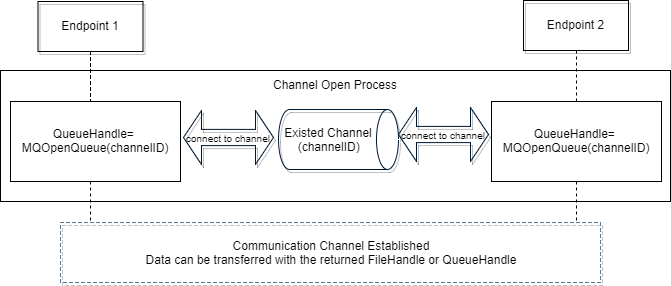
\includegraphics[scale=0.55]{Figures/msmqchannelopen}}
 \caption{Channel Open Process for a Message Queue}
\label{msmqopen}
\end{figure}
    
\subsection{TCP and UDP}
In Windows programming, these two methods shared the same set of APIs regardless the input parameter values and operation behaviour are different. In Windows socket solution, one of the two endpoints is the server while the other one is the client. Table \ref{tcpupdfunctions} lists the functions of a UDP or TCP communication. 
  \begin{table}[H]
        \centering
        \caption{Function List  of events for TCP and UDP}
        \label{tcpupdfunctions}
        \begin{tabular}{|l|l|l|l|l|}
            \hline
             \multirow{2}{*}{\textbf{Event}} &
               \multicolumn{2}{c|}{\textbf{Server Endpoint}} &
               \multicolumn{2}{c|}{\textbf{Client Endpoint}} \\
             \cline{2-5}
              & \textbf{Function}& \textbf{Parameters} & \textbf{Function} & \textbf{Parameters}  \\
             \hline
             \textbf{Channel Open}
             &socket&  RAX: Socket Handle & socket &  RAX: Socket Handle\\
             \hline
                \multirow{2}{*}{{\textbf{Channel Open}}}
              &\multirow{2}{*}{{bind}} &  RCX: Socket Handle & \multirow{2}{*}{connect} &  RCX: Socket Handle\\
              \cline{3-3} \cline{5-5}
             &&  RDX: Server Address $\&$ Port &  &  RDX: Server Address $\&$ Port\\
            \hline
                \multirow{3}{*}{{\textbf{Channel Open}}}
             &\multirow{3}{*}{{accept}} &  RAX: New Socket Handle && \\
              \cline{3-3} 
             &&  RCX:  Socket Handle &  & \\
             \cline{3-3} 
             &&  RDX: Client Address $\&$ Port &  &  \\
            \hline
             \multirow{2}{*}{{\textbf{Send}}}
             &\multirow{2}{*}{send} &  RCX: New Socket Handle & \multirow{2}{*}{send} &  RCX: Socket Handle\\
              \cline{3-3} \cline{5-5}
             &&  RDX: Buffer Address &  &  RDX: Buffer Address\\
           \hline
              \multirow{2}{*}{{\textbf{Receive}}}
             & \multirow{2}{*}{recv}&  RCX: New Socket Handle & \multirow{2}{*}{recv} &  RCX: Socket Handle\\
              \cline{3-3} \cline{5-5}
              &&  RDX: Buffer Address &  &  RDX: Buffer Address\\
            \hline
          {{\textbf{Channel Close}}}&
            {closesocket} & {RCX: New Socket Handle} &{closesocket} & {RCX: Socket Handle}\\
            \hline
        \end{tabular}
    \end{table} 
    
The communication channel is set up by both of the endpoints. The function \textit{socket} should be called to create their own socket on both endpoints. After the sockets are created, the server endpoint binds the socket to its service address and port by calling the function \textit{bind}. Then the server endpoint calls the function  \textit{accept} to accept the client connection. The client will call the function \textit{connect} to connect to the server. When the function \textit{accept} return successfully, a new socket handle will be generated and returned for further data transfer between the server endpoint and  the connected client endpoint. After all these operations are performed successfully, the channel is established and the data transfer can start. During the channel open stage, server endpoint has two socket handles, the first one is used to listen to the connection from the client, while the second one is created for real data transfer. Figure\ref{channelopen2} shows the channel open process for TCP and UDP.
    
\begin{figure}[H]
\centerline{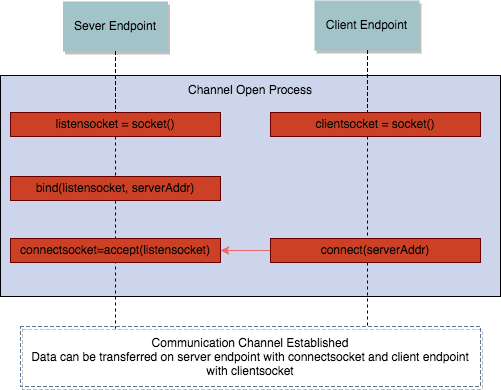
\includegraphics[scale=0.55]{Figures/tcpudpchannelopen}}
 \caption{Channel Open Model for TCP and UDP}
\label{channelopen2}    
\end{figure}

\section{Communication Event Locating in Assembly Execution Traces}
The goal of this research is to identify the communications from the dual-trace and present them to the user. The identification of all events of the communications from the execution trace would be the first step. Last section concludes communication events including system function names, parameters and the function calls relationship. This section will 1) discuss the basis of the execution traces. and 2) conclude how to retrieve the event information from the execution traces.

\subsection{Assembly Execution Trace}
The dual-trace being analysed are in assembly level. One dual-trace contains two execution traces. There is no timing information of these two traces which means we don't know the timestamps of the events of these two traces and can not match the events from both sides by time sequence. However the captured instructions in the trace are ordered in execution sequence. The execution traces contain all executed instructions as well as the corresponding changed memory by each instruction. Additionally, system calls are also captured by instruction id, which means if .dll or .exe files are provided, the system function calls can be identified with function names. Memory states can be reconstructed from the recorded memory changes to get the data information of the communication. 

\subsection{Event Information Retrieval}
For simplification, each function call is treated as an event. A function call in the trace starts from the function call instruction to the function return instruction. The input parameters' value and input buffer content should be retrieved from the memory state of the the function call instruction line while the return value, output parameters' value and output buffer content should be retrieved from the memory state of the function return instruction line. Tables in section \ref{windows} indicate all the functions of the communication methods as well as the concerned parameters. Following the windows calling convention, the concerned parameter value or buffer address can be found in the corresponding register or stack positions. The buffer content can be found in the memory address in the reconstructed memory state. 


